
\begin{frame}{\citetitle{MarcoNuno_Revista_2022_03_00}$^*$  (1)}
\begin{columns}
\begin{column}{0.6\textwidth}
	\begin{itemize}
		\item Una solución al problema de manejo de desechos es el reciclado
        \item Específicamente, la separación por color de una botella es de utilidad para su correcto manejo
        \item Se propone un sistema para clasificar botellas en una banda transportadora
        \item El nucleo del sistema es una arquictectura hardware que realiza tareas de visión para clasificación tiempo real 
	\end{itemize}
\end{column}
\begin{column}{0.4\textwidth}  
\begin{center}
     \begin{tabular}{cc}
         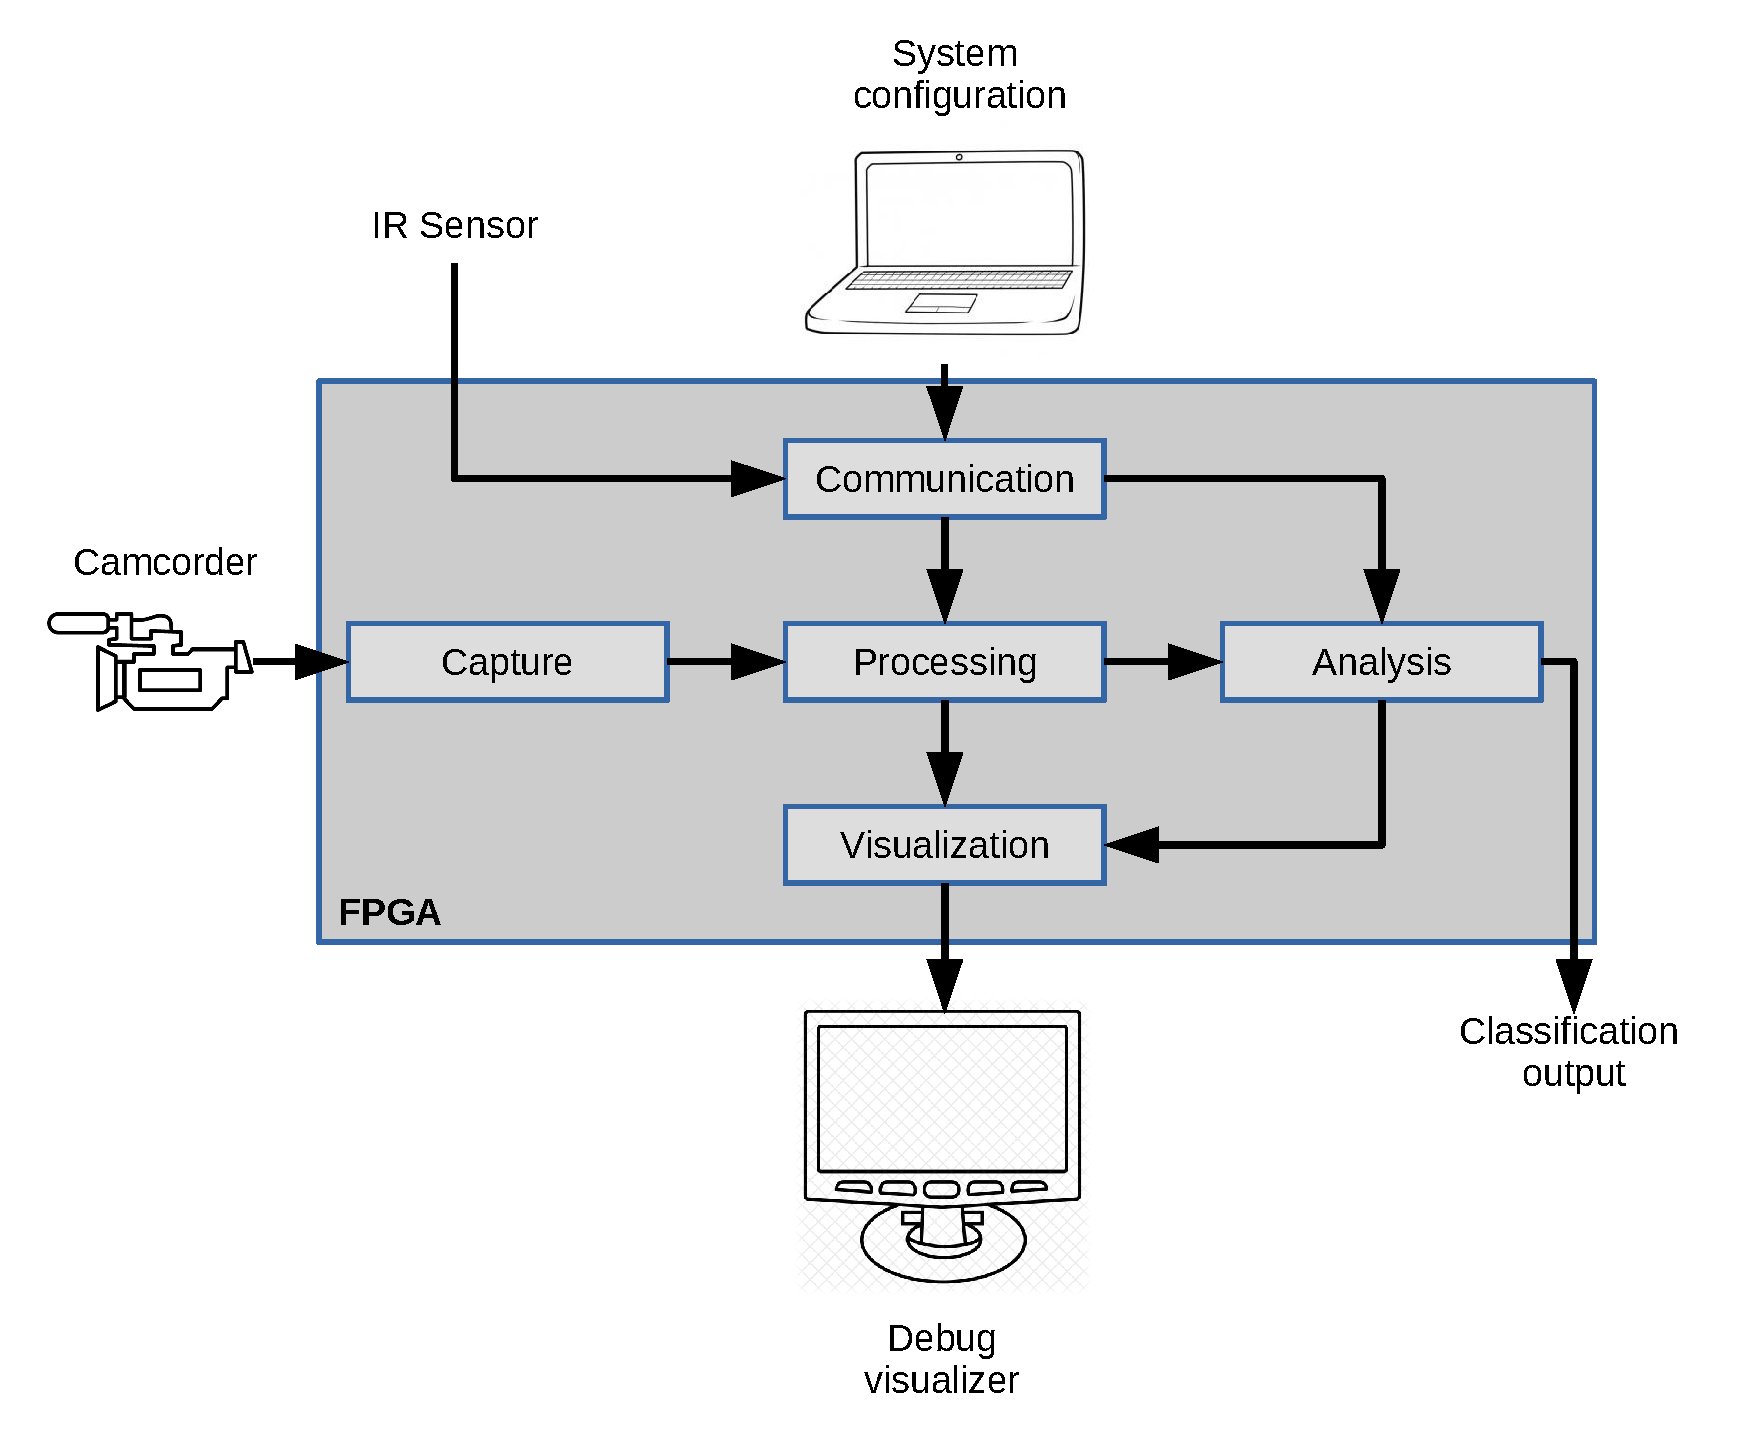
\includegraphics[width=0.98\textwidth]{2022_BottleClassifier/figs/MainModules.pdf}\\         
      \end{tabular}
\end{center}
\end{column} 
\end{columns} 
\footfullcite*{MarcoNuno_Revista_2022_03_00}
\end{frame}


\begin{frame}{\citetitle{MarcoNuno_Revista_2022_03_00} (2)}
\begin{columns}
\begin{column}{0.5\textwidth}

Materiales:
\begin{itemize}
        \item Sensor óptico de presencia
        \item Tarjeta FPGA - Spartan 6 Industrial Video Processing Kit
        \item Cámara con salida HDMI
        \item Monitor para depuración
        \item Circuitos para activar actuadores de separación de botellas
	\end{itemize}
\end{column}
\begin{column}{0.5\textwidth}  
\begin{center}
     \begin{tabular}{c}
         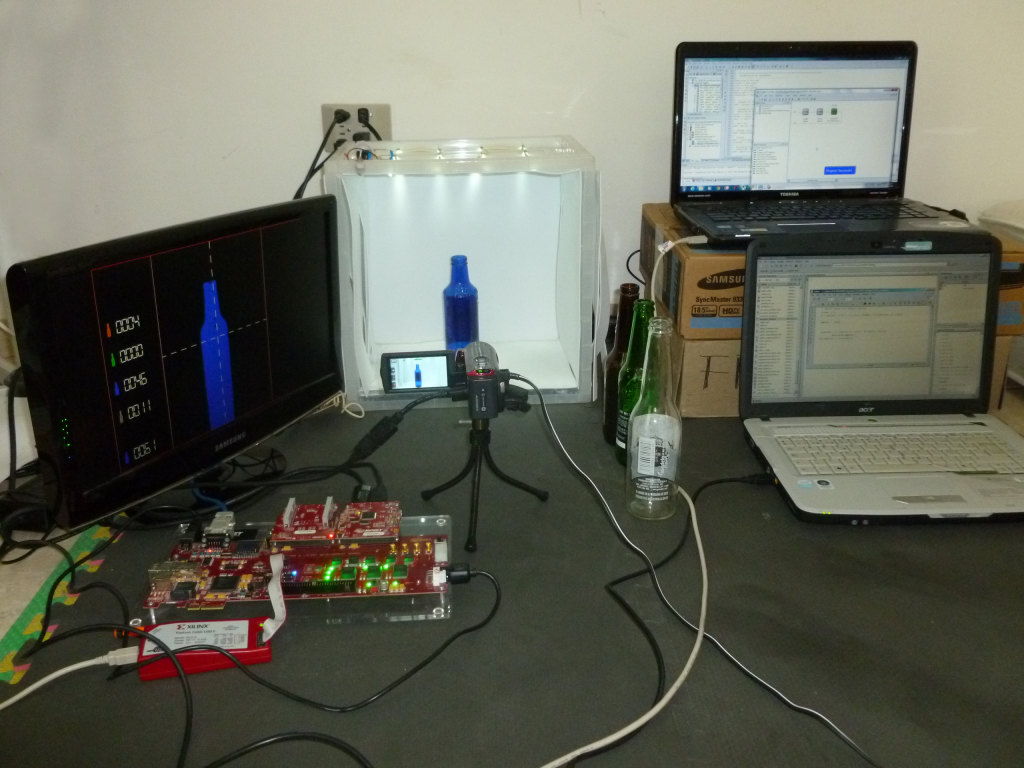
\includegraphics[width=0.98\textwidth]{2022_BottleClassifier/figs/cap4_setup.png}\\
          \end{tabular}
\end{center}
\end{column} 
\end{columns} 
\end{frame}

\begin{frame}{\citetitle{MarcoNuno_Revista_2022_03_00} (3)}
El nucleo del sistema propuesto es el módulo del sistema de visión, que ejecuta las siguientes tareas:
\begin{itemize}
        \item Aplicar filtros (promediado y de mediana)
        \item Convertir de Color a HSV
        \item Efectuar operaciones morfológica
        \item Calcular histograma
        \item En base a reglas previamente definidas, clasifica la botella por color
	\end{itemize}

%\begin{center}
% 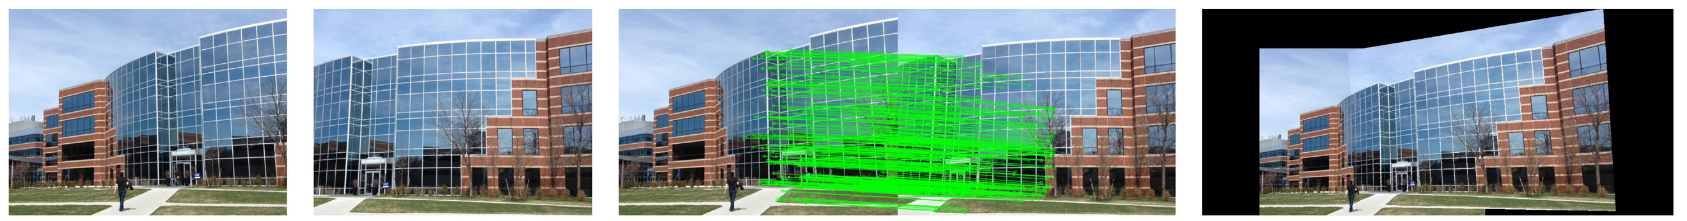
\includegraphics[width=0.95\textwidth]{2022_ConteoOstioncitos/figs/ImageMatchingAndRegistration.png}
%\end{center}

\end{frame}


\begin{frame}{\citetitle{MarcoNuno_Revista_2022_03_00} (4)}
\begin{columns}
\begin{column}{0.6\textwidth}
\begin{itemize}
\item Una vez que el sensor óptico detecta la botella, inicia el procesamiento de imágen
\item Cuando el procesamiento de imágen termina, arroja como resultado la clasificación de la botella
\item Se incrementa un contador de cada botella y se muestra en la pantalla de depuración
\item Es posible configurar los umbrales, para separar botellas de diferente color diferentes
\end{itemize}
\end{column} 
\begin{column}{0.3\textwidth}
 \begin{tabular}{c}
    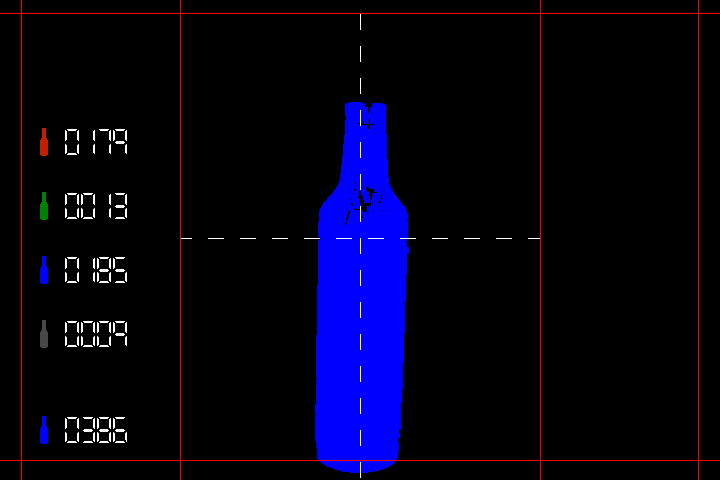
\includegraphics[width=0.98\textwidth]{2022_BottleClassifier/figs/cap4_dispfinal.png}\\
    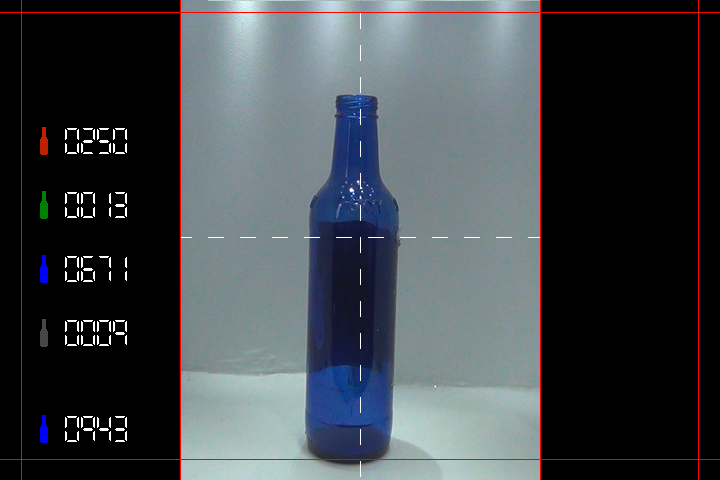
\includegraphics[width=0.98\textwidth]{2022_BottleClassifier/figs/cap4_disporiginal.png}
  \end{tabular}
\end{column} 
\end{columns} 

\end{frame}




